\begin{figure}
    \centering
    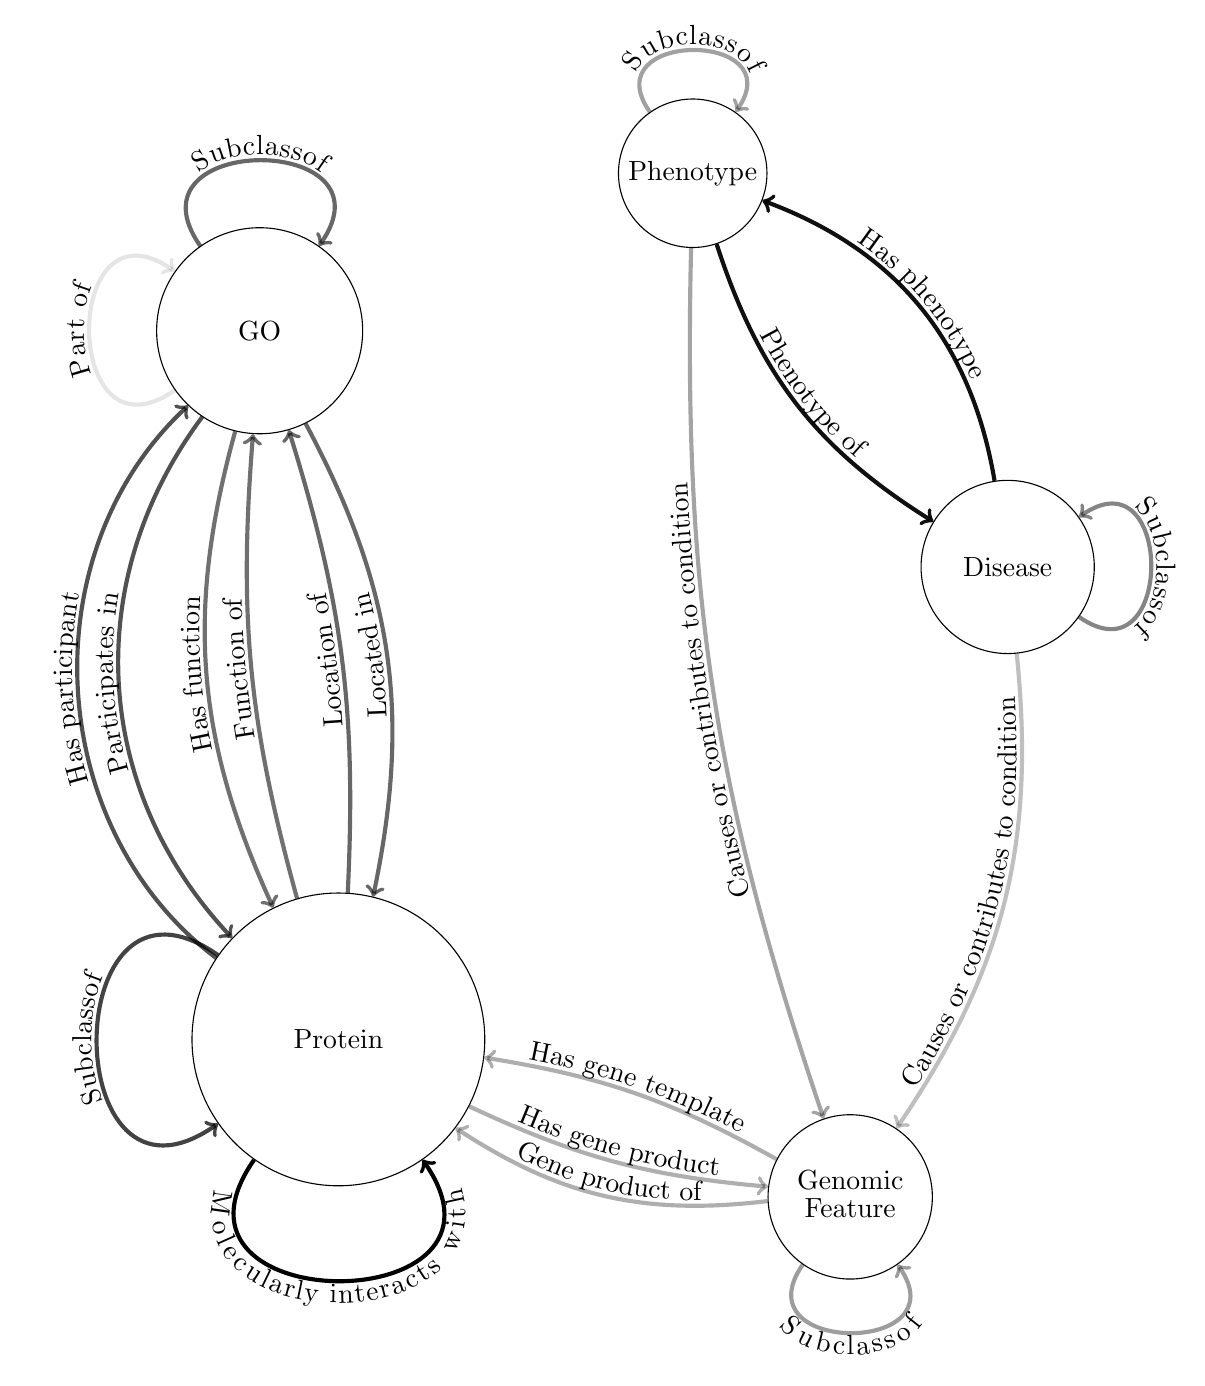
\begin{tikzpicture}
    \usetikzlibrary{decorations.text}

    \begin{scope}[xshift=1cm]
        % Nodes
        \node[circle, draw, fill=none, minimum size=3.718cm, inner sep=0pt] (Protein) at (-4,-3) {Protein};
        \node[circle, draw, fill=none, minimum size=2.617cm, inner sep=0pt] (GO) at (-5,6) {GO};
        \node[circle, draw, fill=none, minimum size=2.200cm, inner sep=0pt] (Disease) at (4.5,3) {Disease};
        \node[circle, draw, fill=none, minimum size=2.087cm, inner sep=0pt] (GenomicFeature) at (2.5,-5) {\begin{tabular}{c}Genomic\\[-0.5ex]Feature\end{tabular}};
        \node[circle, draw, fill=none, minimum size=1.886cm, inner sep=0pt] (Phenotype) at (0.5,8) {Phenotype};

        % Edges with curved labels
            \draw[->, line width=1.5pt, opacity=0.937927] (Disease) to[bend right=30] (Phenotype);
            \path[decorate, decoration={text along path, text align=center, raise=2pt, text={Has phenotype}}] (Phenotype) to[bend left=30] (Disease);

            \draw[->, line width=1.5pt, opacity=1.000000] (Protein) to[out=235, in=305, looseness=3] (Protein);
            \path[decorate, decoration={text along path, text align=center, raise=-8pt, text={Molecularly interacts with}}] (Protein) to[out=235, in=305, looseness=3](Protein);

            \draw[->, line width=1.5pt, opacity=0.478617] (Disease) to[out=-35, in=35, looseness=3] (Disease);
            \path[decorate, decoration={text along path, text align=center, raise=2pt, text={Subclassof}}] (Disease) to[out=35, in=-35, looseness=3] (Disease);

            \draw[->, line width=1.5pt, opacity=0.596164] (GO) to[out=125, in=55, looseness=3] (GO);
            \path[decorate, decoration={text along path, text align=center, raise=2pt, text={Subclassof}}] (GO) to[out=125, in=55, looseness=3] (GO);

            \draw[->, line width=1.5pt, opacity=0.383857] (GenomicFeature) to[out=235, in=305, looseness=3] (GenomicFeature);
            \path[decorate, decoration={text along path, text align=center, raise=-8pt, text={Subclassof}}] (GenomicFeature) to[out=235, in=305, looseness=3] (GenomicFeature);

            \draw[->, line width=1.5pt, opacity=0.367024] (Phenotype) to[out=125, in=55, looseness=3] (Phenotype);
            \path[decorate, decoration={text along path, text align=center, raise=2pt, text={Subclassof}}] (Phenotype) to[out=125, in=55, looseness=3] (Phenotype);

            \draw[->, line width=1.5pt, opacity=0.735558] (Protein) to[out=145, in=215, looseness=3] (Protein);
            \path[decorate, decoration={text along path, text align=center, raise=2pt, text={Subclassof}}] (Protein) to[out=215, in=145, looseness=3] (Protein);

            \draw[->, line width=1.5pt, opacity=0.561965] (Protein) to[bend left=10] (GO);
            \path[decorate, decoration={text along path, text align=center, raise=2pt, text={Function of}}] (Protein) to[bend left=10] (GO);


            \draw[->, line width=1.5pt, opacity=0.937927] (Phenotype) to[bend right=20] (Disease);
            \path[decorate, decoration={text along path, text align=center, raise=2pt, text={Phenotype of}}] (Phenotype) to[bend right=20] (Disease);

            \draw[->, line width=1.5pt, opacity=0.316749] (GenomicFeature) to[bend right=10] (Protein);
            \path[decorate, decoration={text along path, text align=center, raise=2pt, text={Has gene template}}] (Protein) to[bend left=10] (GenomicFeature);

            \draw[->, line width=1.5pt, opacity=0.561965] (GO) to[bend right=20] (Protein);
            \path[decorate, decoration={text along path, text align=center, raise=2pt, text={Has function}}] (Protein) to[bend left=20] (GO);

            \draw[->, line width=1.5pt, opacity=0.681528] (Protein) to[bend left=50] (GO);
            \path[decorate, decoration={text along path, text align=center, raise=2pt, text={Has participant}}] (Protein) to[bend left=50] (GO);

            \draw[->, line width=1.5pt, opacity=0.311908] (Protein) to[bend right=10] (GenomicFeature);
            \path[decorate, decoration={text along path, text align=center, raise=2pt, text={Has gene product}}] (Protein) to[bend right=10] (GenomicFeature);

           

            \draw[->, line width=1.5pt, opacity=0.595817] (Protein) to[bend right=10] (GO);
            \path[decorate, decoration={text along path, text align=center, raise=2pt, text={Location of}}] (Protein) to[bend right=10] (GO);

            \draw[->, line width=1.5pt, opacity=0.595822] (GO) to[bend left=20] (Protein);
            \path[decorate, decoration={text along path, text align=center, raise=2pt, text={Located in}}] (Protein) to[bend right=20] (GO);

            \draw[->, line width=1.5pt, opacity=0.681523] (GO) to[bend right=40] (Protein);
            \path[decorate, decoration={text along path, text align=center, raise=2pt, text={Participates in}}] (Protein) to[bend left=40] (GO);

            \draw[->, line width=1.5pt, opacity=0.250632] (Disease) to[bend left=20] (GenomicFeature);
            \path[decorate, decoration={text along path, text align=center, raise=2pt, text={Causes or contributes to condition}}] (GenomicFeature) to[bend right=20] (Disease);

            \draw[->, line width=1.5pt, opacity=0.356471] (Phenotype) to[bend right=10] (GenomicFeature);
            \path[decorate, decoration={text along path, text align=center, raise=2pt, text={Causes or contributes to condition}}] (GenomicFeature) to[bend left=10] (Phenotype);

            \draw[->, line width=1.5pt, opacity=0.311908] (GenomicFeature) to[bend left=20] (Protein);
            \path[decorate, decoration={text along path, text align=center, raise=2pt, text={Gene product of}}] (Protein) to[bend right=20] (GenomicFeature);

            \draw[->, line width=1.5pt, opacity=0.100000] (GO) to[out=215, in=145, looseness=3] (GO);
            \path[decorate, decoration={text along path, text align=center, raise=2pt, text={Part of}}] (GO) to[out=215, in=145, looseness=3] (GO);   \end{scope}
    \end{tikzpicture}

    \caption{A hypergraph representation of the underlying knowledge graph, having hypernodes representing the possibile node types and hyperedges for the most frequent edge predicates. The hypernodes' size and the hyperedges' opacity are logarithmic in the amount of node types and edge predicates respectively.}
    \label{fig:kg_hypergraph}
\end{figure}